% MiKTeX (LaTeX) Beamer Presentation template
% Author: Carl Schneider
% University TUDelft
% November 2011
% Simple example (without TOC)

\documentclass{beamer}


% for matlab plots
\usepackage{pgfplots}
% and optionally (as of Pgfplots 1.3):
\pgfplotsset{compat=newest}
\pgfplotsset{plot coordinates/math parser=false}
\newlength\figureheight
\newlength\figurewidth

\usepackage{setspace}

% Necessary definitions:
\setbeamersize{sidebar width left=0.5cm}
\usepackage[english]{babel}
\usepackage{tikz}
\newcommand{\field}[1]{\mathbb{#1}}
\newcommand{\Zset}{\field{Z}}
\mode<presentation>
{\usetheme{Boadilla} % This theme will be changed into the TUDelft lay-out
  \setbeamercovered{transparent}
}
\definecolor{tudblue}{HTML}{0092DF} % definition TUDelft blue color
\definecolor{white}{rgb}{1,1,1} % definition TUDelft blue color
\setbeamercolor{structure}{fg=tudblue}
\setbeamercolor{palette primary}{fg=white,bg=tudblue!85}       % Right field
\setbeamercolor{palette secondary}{fg=white,bg=tudblue!85}     % Middle field
\setbeamercolor{palette tertiary}{fg=tudblue!85,bg=tudblue!85} % Left field
\setbeamersize{text margin left=1cm}
\setbeamersize{text margin right=1cm}

%---------------------------------------------------------------------------------
%  Take attention for the parts you may change. See the comment lines with: %>>>
%---------------------------------------------------------------------------------

%>>> You may change the text in this part {Between brackets}:
%>>> This is for the Title page:
\newcommand*\titel{FF-Replan \& RFF} % On titelpage and in footer on every page
\newcommand*\subkop{A Baseline for Probabilistic Planning \\ Incremental Plan Aggregation for Generating Policies in MDPs} % In blue color
\newcommand*\naam{Imara Speek \& Arian Stolwijk}
\newcommand*\afdeling{}

\setbeamertemplate{navigation symbols}{}

\setbeamercolor{section in head/foot}{fg=white,bg=tudblue}

\setbeamertemplate{footline}{
  \begin{beamercolorbox}[wd=\paperwidth,leftskip=0.5cm,rightskip=0.5cm]{section in head/foot}
    \inserttitle \hfill \insertframenumber{} / \inserttotalframenumber
  \end{beamercolorbox}
}

\let\origframetitle=\frametitle
\renewcommand\frametitle[1]{\origframetitle{\textbf{\large{\textrm{#1}}}}}

%==============================================================
%%% DO NOT CHANGE this part below %%%
%%% Title Page (belongs to the theme)%%%
% Necessary part for the theme:
\title{\titel} % This title also appears in the TUDelft bar on the next pages
\author[]{\naam}
\institute[]{\subkop \\ TU Delft}
\date[]{\today}
\tikzset{textlabel/.style={color=white}}
\beamertemplatetransparentcovereddynamicmedium

%==============================================================
%%% DO NOT CHANGE this part below, except maybe the folder where you placed the "TUDelft bies"
\begin{document}
% Adjusting boadilla theme lay-out to TUDelft lay-out:
\setbeamertemplate{sidebar left}  % blue square left above
{\vfill
\rlap{%\hskip0.1cm

\includegraphics[scale=0.33]{TUDelft/beamer-tudelft-bies.jpg} }
\vskip-5pt}
%==============================================================

% Title page
%%% This is the first frame of the presentation (Title Page).
%%% DO NOT CHANGE this part except maybe the comment signs in case of a background photo
%%% and the place and name of the photo
\begin{frame}[label=titlepage]
    \begin{tikzpicture} [remember picture, overlay]
        \node [shift={(0.5 cm,-5.35cm)}]  at (current page.north west)
        {
        \begin{tikzpicture}[remember picture, overlay]
            %%% These 2 coming lines you may uncomment if you want to have a photo on the background(2198x1480pixels) of the title page

            \node [shift={(-0.14cm,5.56cm)},right] at (current page.south west)
            {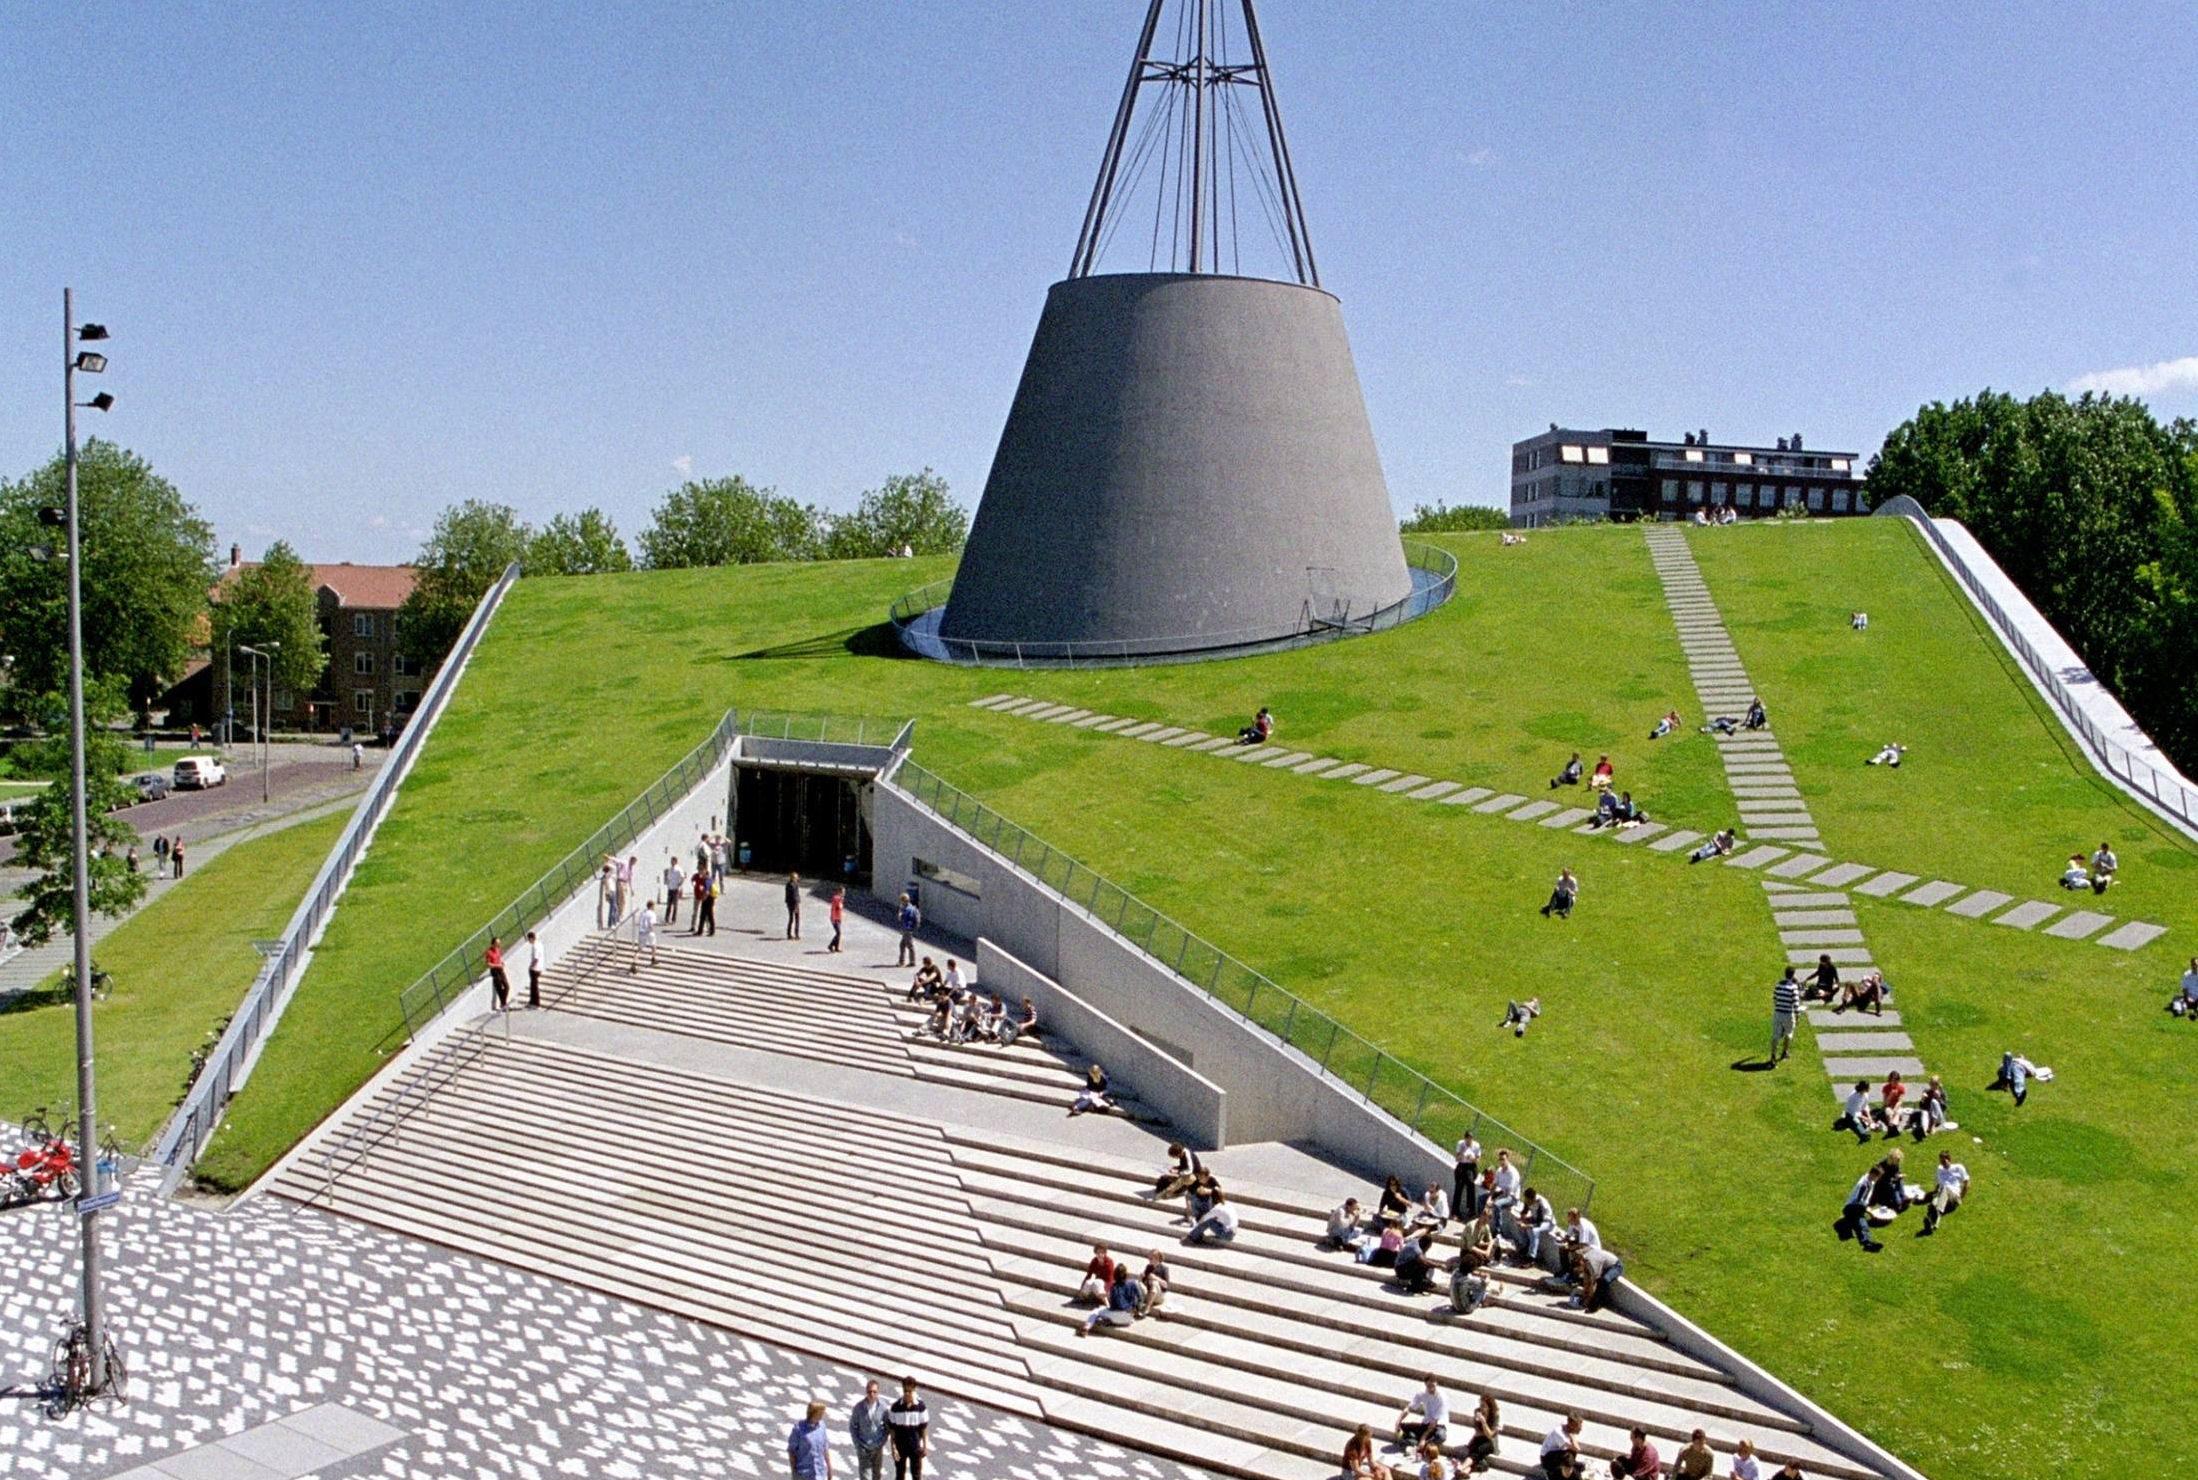
\includegraphics[height=8.65cm]{TUDelft/background-titlepage.jpg}};

            % hide the navigation things.
            \fill [cyan!95!black!70!blue] (0,2.9) -- (0,5.35) -- (-.5,5.35) -- (-.5,2.9) -- cycle ;%squareNorthWest
            \draw [fill=black] (0,0) -- (11,0) -- (11,2.9) -- (0,2.9) -- cycle ;
            %\fill [fill=cyan!65!blue!80] (7,-3.9) -- (12.4,-3.9) -- (12.4,-3.65) -- (7,-3.65) -- cycle;

            \node [shift={(0.8cm,-3.1cm)},textlabel,right,text width=10cm]  at (current page.north west) {\textbf{\large{\textrm{\titel}}}};
            \node [shift={(0.8cm,-4cm)},textlabel,cyan!95!black!70!blue,right,text width=10cm]  at (current page.north west)
            {\textbf{\large{\scriptsize \textrm{\begin{spacing}{0.9}\subkop \end{spacing}}}}};
            \node [shift={(0.8cm,-4.6cm)},textlabel,right]  at (current page.north west)
            {\normalsize{\naam}};
            \node [shift={(0.8cm,-5cm)},textlabel,right]  at (current page.north west)
            {\normalsize{\today}};
        \end{tikzpicture}};
    \end{tikzpicture}
\end{frame}
%==============================================================

\begin{frame}
  \frametitle{Content of presentation}

\end{frame}

\begin{frame}
  \frametitle{Planners}

  What is a Planner?

  \begin{itemize}
    \item From \alert{initial state}
    \item To \alert{Goal state}
    \item Through \alert{Actions}
  \end{itemize}

\end{frame}

\begin{frame}
  \frametitle{Examples of a Planning Problem}

  \begin{tabular}{c c}
    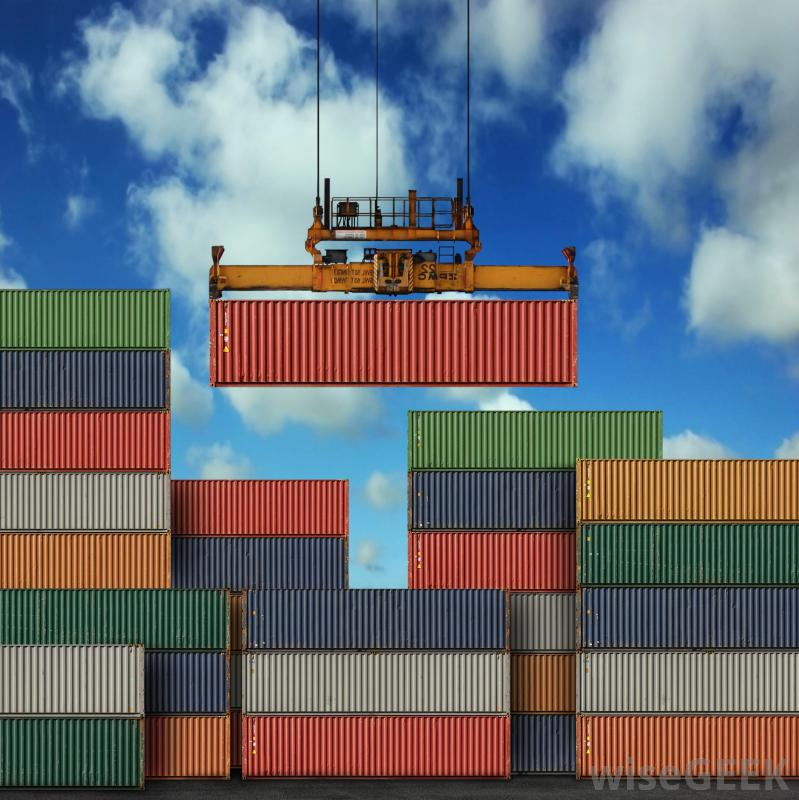
\includegraphics[width=3.5cm]{images/containers.jpg}     &
    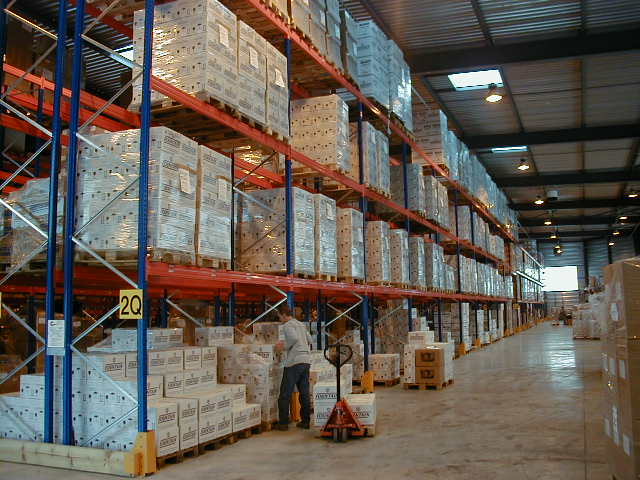
\includegraphics[width=3.5cm]{images/inventory.jpg}      \\
    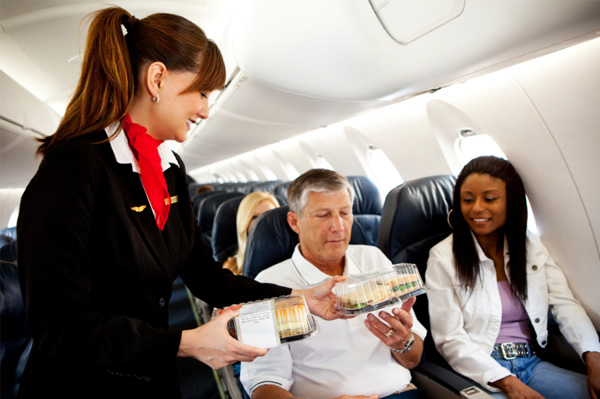
\includegraphics[width=3.5cm]{images/airplane-food.jpg}  &
    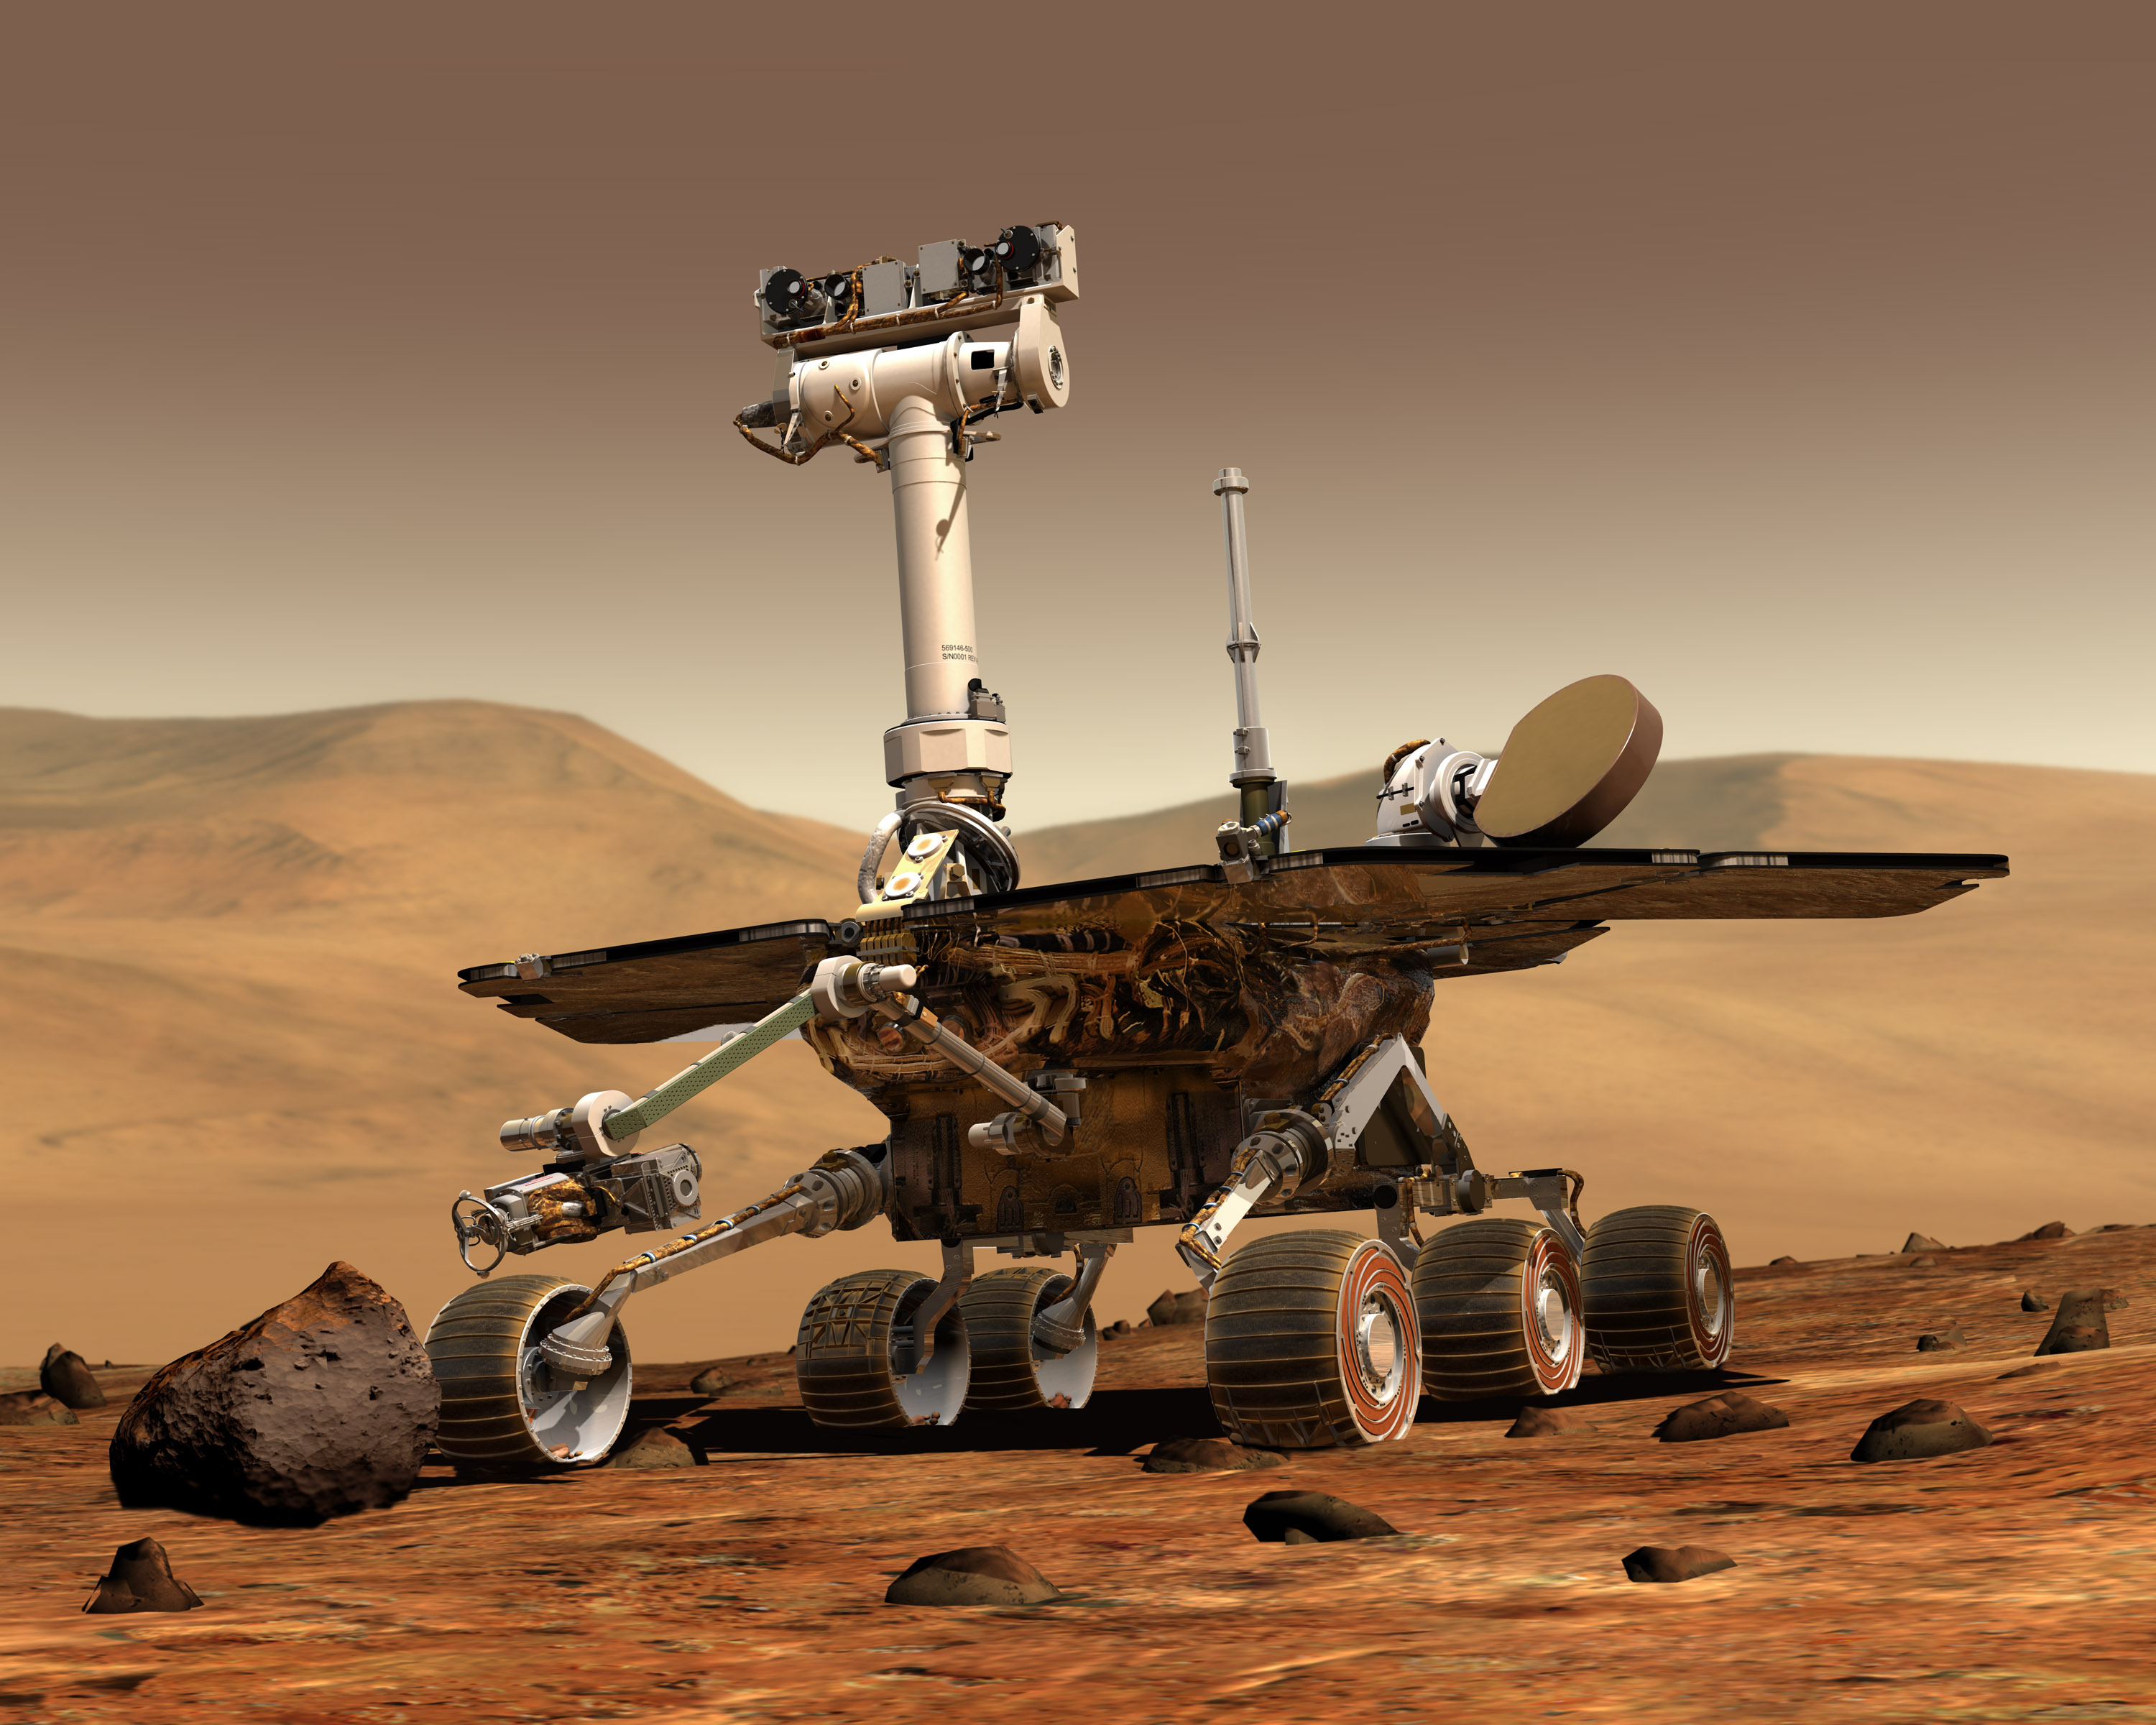
\includegraphics[width=3.5cm]{images/mars-rover.jpg}
  \end{tabular}

\end{frame}

\begin{frame}
  \frametitle{Classical Planning Example}

  \begin{columns}
    \column{0.3\textwidth}
    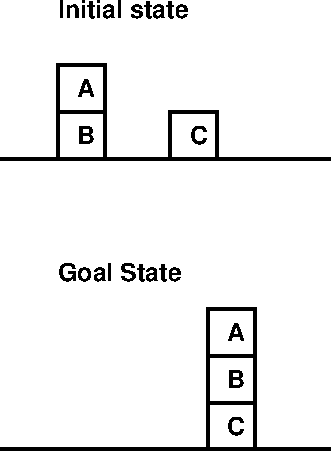
\includegraphics[width=\textwidth]{../presentation-plan/blocksworld.pdf}

    \column{0.7\textwidth}

    \begin{itemize}
      \item From initial state to goal state?
      \item Create a planning plan.
      \item Assumptions:
        \begin{itemize}
          \item Determinism
          \item Full observability
          \item Reachability goals
        \end{itemize}
    \end{itemize}
  \end{columns}

\end{frame}

\begin{frame}
  \frametitle{Uncertainty}

  \emph{``Uncertainty applies to predictions of future events, to physical
  measurements that are already made, or to the unknown. Uncertainty arises in
  partially observable and/or stochastic environments, as well as due to
  ignorance and/or indolence''}

  \vspace{2cm}

  \tiny{http://en.wikipedia.org/wiki/Uncertainty}

\end{frame}


\begin{frame}
  \frametitle{Planning with Uncertainty}

  \begin{columns}
    \column{0.25\textwidth}
    \uncover<1> {Meet my plant}
    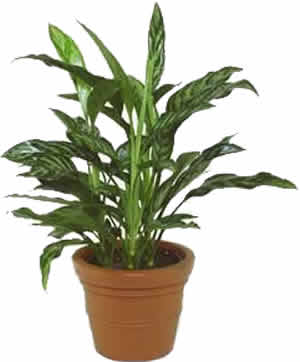
\includegraphics[width=\textwidth]{images/plant.jpg}

    \column{0.75\textwidth}
    \uncover<2->{%

      How to plan when to water the plant?

      \begin{itemize}
        \item Uncertainty from Wind
        \item Sunlight
        \item Water
      \end{itemize}
    }
  \end{columns}

  \vspace{1cm}
  \uncover<3-> {What if picking up a block fails?}

\end{frame}

\begin{frame}
  \frametitle{Markov Decision Processes}

  \begin{itemize}
    \item Very much like a Classical Planner
    \item \alert{except} each action has a \alert{probability}
      \begin{itemize}
        \item \alert{Stochastic}
        \item Full observability
        \item Reachability goals
      \end{itemize}
    \item For example in the Blocksworld: The Pick Up action might fail.
  \end{itemize}

\end{frame}

\begin{frame}
  \frametitle{Historical background information}

  \begin{columns}
    \column{0.8\textwidth}

    \begin{itemize}
      \item 1970s: STRIPS
      \item 1995: Graphplan
      \item 2000: FastForward (FF)
      \item 2004: FF-Replan
      \item 2010: RFF
      \item 2014:~?
    \end{itemize}

    \column{0.2\textwidth}
    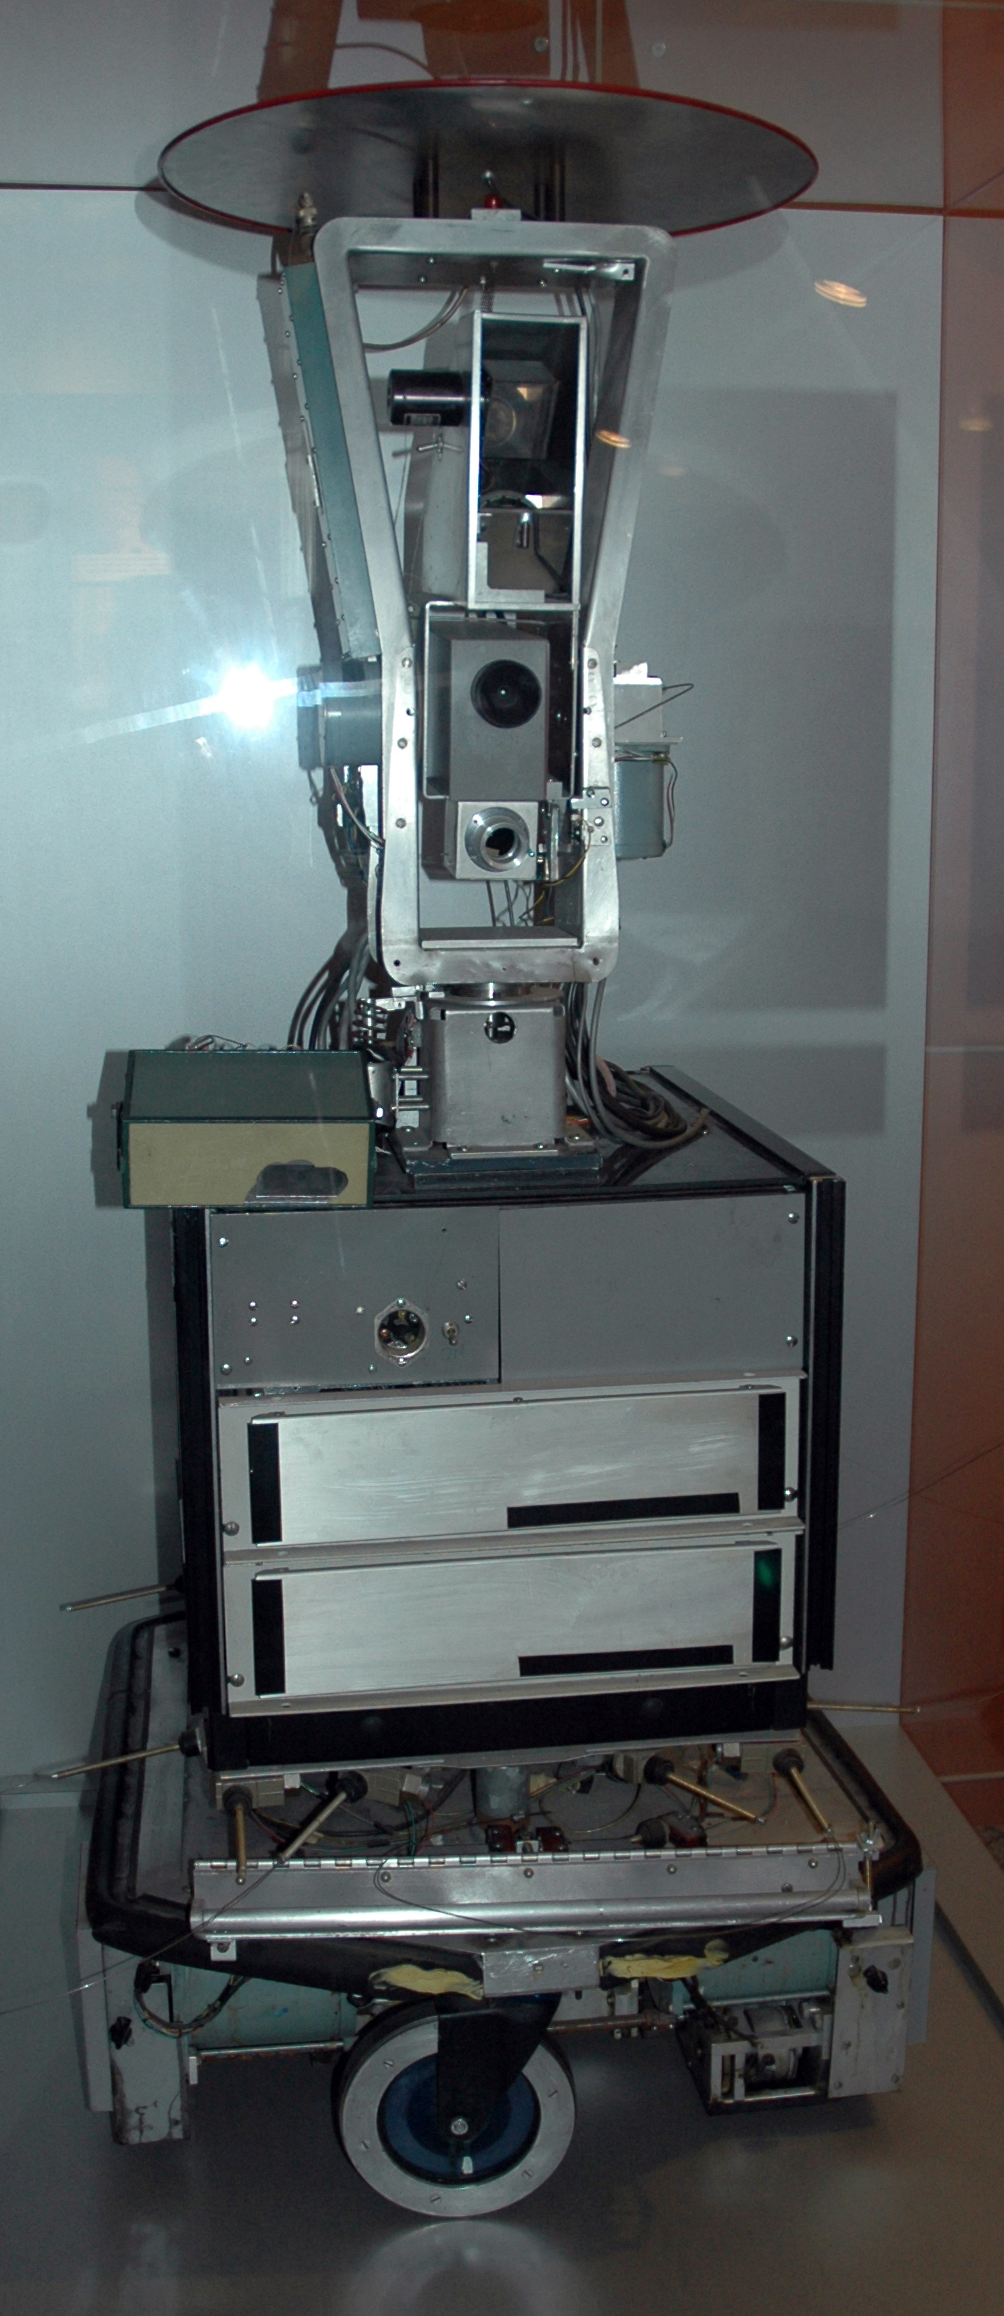
\includegraphics[width=\textwidth]{images/shakey.png}

  \end{columns}
\end{frame}

\begin{frame}
  \frametitle{FF Planner (2001)}

  ``We have presented an approach to domain independent planning that, \emph{at
  the time being}, outperforms all existing technology on the majority of the
  currently available benchmark domains.''

\end{frame}

\begin{frame}
  \frametitle{FF Planner (2001)}

  Inspired by three new approaches in plan generation during that time:

  \begin{itemize}
    \item Planning graphs
    \begin{itemize}
      \item Nodes are actions and atomic facts arranged into alternate levels
      \item Edges from atomic facts to actions represents conditions
      \item Edges from actions to atomic facts represent true or false
    \end{itemize}
    \item Planning as a satisfiability method
    \item Heuristic search planning approach
  \end{itemize}
\end{frame}

\begin{frame}
  \frametitle{FF Planner (2001)}

  Relies on a

  \begin{itemize}
    \item Forward state space search that combines hill-climbing and systematic search
    \item Heuristic estimating goal distances by ignoring delete lists - relaxed GRAPHPLAN
  \end{itemize}

\end{frame}

\begin{frame}
  \frametitle{FF Planner (2001)}

  Insert image on search state, enforced hill climbing, call relaxed Graphplan,
  inform search with goal distance estimate and maybe promising successors,
  solution plan or fail, possible search from scratch using hast table with
  visited states

\end{frame}

\begin{frame}
  \frametitle{FF Planner (2001)}
    Same image

  To avoid wasting time in the presence of goal ordering:

  \begin{itemize}
    \item Goal deletion
    \item Goal agenda techniques
  \end{itemize}

\end{frame}

\begin{frame}
  \frametitle{Discussing the FF planner}

\begin{itemize}
\item  Perks
  \begin{itemize}
    \item No efficient algorithmic methods are possible for PSPACE-complete planning, inspired to focus on being efficient on a restricted subclass
    \item Most domains in the IPCC are simple in their structure and can be easily solves using greedy algorithms like FF
  \end{itemize}
\item Criticism
  \begin{itemize}
    \item Methods are motivated by observing example domains - might influence the completeness
    \item Pruning techniques are incomplete
    \item FF behaves poorly in domains with many dead-ends
    \item Solving these tasks with complete best-first search exhaust the memory for larger instances
  \end{itemize}
\end{itemize}
\end{frame}


\begin{frame}
  \frametitle{Planning under uncertainty: FF-Replan}

  \begin{itemize}
    \item Problem
      \begin{itemize}
        \item MDPs have been the standard for probabilistic planning algorithms
        \item MDPs can be computationally intensive
        \item typically enumerate the entire state and action space
      \end{itemize}
    \item Motivation for the FF planner
      \begin{itemize}
        \item Technological development within processing units
        \item Relying on search introduces speed and efficiency
      \end{itemize}
  \end{itemize}
\end{frame}

\begin{frame}
  \frametitle{FF-Replan - details of the solution}

  \begin{itemize}
    \item The planning problem
      \begin{itemize}
        \item a domain description
        \item a goal
        \item an initial state
      \end{itemize}
    \item FF-replan
      \begin{itemize}
        \item Generates a deterministic planning problem
        \item Uses the FF planner to compute a totally-ordered plan
        \item If during execution an unexpected (not in the hash-table) occurs, the process is repeated using this as an initial state
      \end{itemize}
  \end{itemize}
\end{frame}

\begin{frame}
  \frametitle{FF-Replan - details of the solution}

  \begin{itemize}
    \item Determinization
      \begin{itemize}
        \item Single outcome determinization
        \item All-outcomes determinization
      \end{itemize}
   \end{itemize}
\end{frame}

\begin{frame}
  \frametitle{FF-Replan - details of the solution}

  \begin{itemize}
    \item Determinization
    \item Planning
      \begin{itemize}
        \item Partial state-action mapping using an initial empty hash-table
        \item Unexpected states are determinized and the synthesized plan (by FF) is put in the hash table
      \end{itemize}

      \emph{insert image how hash table is filled}

   \end{itemize}
\end{frame}

\begin{frame}
  \frametitle{FF-Replan - Critism}

  \begin{itemize}
    \item Shortcomings
      \begin{itemize}
        \item Probabilistic effects are treated as equal
          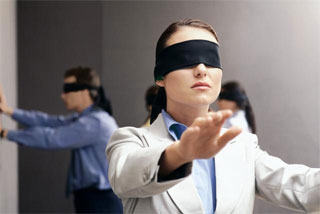
\includegraphics[scale=0.5]{images/blindfold.jpg}
      \end{itemize}
    \item Means of improvement
  \end{itemize}
\end{frame}

\begin{frame}
  \frametitle{FF-Replan - Critism}

  \begin{itemize}
    \item Shortcomings
      \begin{itemize}
        \item Probabilistic effects are treated as equal
        \item Only works well if the outcomes are likely
          
\includegraphics[scale=0.3]{images/direction-road-maze.jpg}
        \end{itemize}
    \item Means of improvement
  \end{itemize}
\end{frame}

\begin{frame}
  \frametitle{FF-Replan - Critism}

  \begin{itemize}
    \item Shortcomings
      \begin{itemize}
        \item Probabilistic effects are treated as equal
        \item Only works well if the outcomes are likely
          
\includegraphics[scale=0.01]{images/direction-road-maze.jpg}
      \end{itemize}
    \item Means of improvement
      \begin{itemize}
        \item
      \end{itemize}
   \end{itemize}
\end{frame}

\begin{frame}
  \frametitle{Planning under uncertainty: RFF}

  \begin{itemize}
    \item Problem
      \begin{itemize}
        \item MDPs can be computationally intensive
        \item MDPs typically enumerate the entire state and action space
      \end{itemize}
    \item Motivation
      \begin{itemize}
        \item FF-Replan showed MDP determinization and replanning techniques
        \item However, it stops after the first computed path to a goal
        \item May generate same path over and over
        \item Does not generate a policy
      \end{itemize}
  \end{itemize}

\end{frame}

\begin{frame}
  \frametitle{RFF Solution}

  \begin{columns}
    \column{0.3\textwidth}
    \only<1> {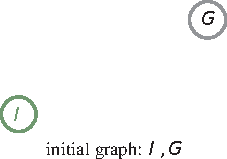
\includegraphics[width=\textwidth]{images/rff-1.pdf}}
    \only<2> {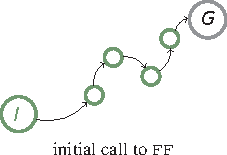
\includegraphics[width=\textwidth]{images/rff-2.pdf}}
    \only<3> {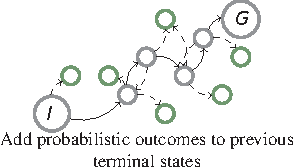
\includegraphics[width=\textwidth]{images/rff-3.pdf}}
    \only<4> {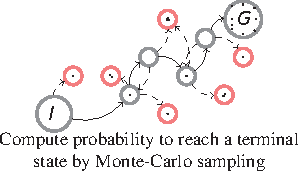
\includegraphics[width=\textwidth]{images/rff-5.pdf}}
    \only<5> {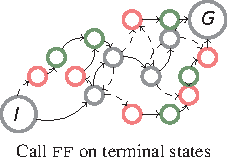
\includegraphics[width=\textwidth]{images/rff-6.pdf}}

    \column{0.7\textwidth}

    \only<1>{%
      \begin{itemize}
        \item Initial state and goal of MDP
        \item Determinization of MDP
          \begin{itemize}
            \item \textsc{MostProbableOutcome} % follows action with highest probability to next state
            \item \textsc{AllOutcomes} % follows all actions to next states
          \end{itemize}
      \end{itemize}
    }
    \only<2>{%
      \begin{itemize}
        \item Use \texttt{FF} to generate initial plan
      \end{itemize}
    }
    \only<3>{%
      \begin{itemize}
        \item Expand structure
      \end{itemize}
    }
    \only<4>{%
      \begin{itemize}
        \item Use Monte-Carlo sampling to compute the probability to reach nodes in the structure
      \end{itemize}
    }
    \only<5>{%
      \begin{itemize}
        \item If the probability of the MC sampling is higher than $\rho$
        \item Then \texttt{FF} is called, which trajectory is merged with the graph
          \begin{itemize}
            \item \texttt{FF} to \textsc{ProblemGoal}
            \item \texttt{FF} to \textsc{RandomGoal}
            \item \texttt{FF} to \textsc{BestGoal}
          \end{itemize}
        \item Then go back expanding structure from terminal states
        \item Or if there are no terminal states with $P_t > \rho$ stop
      \end{itemize}
    }
  \end{columns}

\end{frame}

\begin{frame}
  \frametitle{RFF Results}

  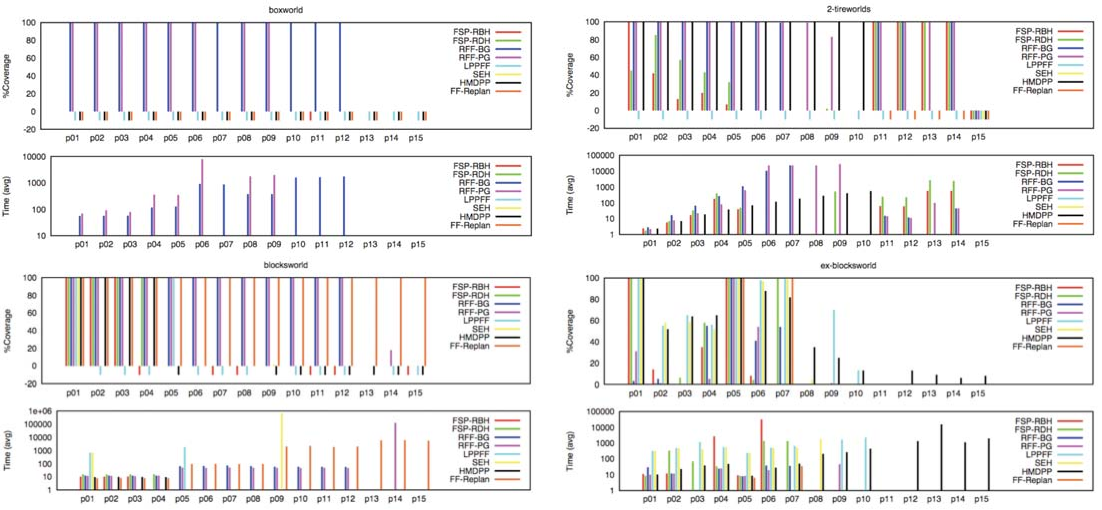
\includegraphics[width=\textwidth]{images/rff-results.pdf}
\end{frame}

\begin{frame}
  \frametitle{RFF Discussion}

  \begin{itemize}
    \item Won the IPC-08 competition in the ``Fully Observable Probabilistic'' track
    \item Probability a sulution is found is $1 - \rho$
    \item $> \rho$ means more replanning
  \end{itemize}

  \setbeamertemplate{itemize items}[square]
  \begin{itemize}
    \item A clear goal must be defined. Does not perform well for the Search-and-Resque domain
    \item If a solution is found, it is correct, but might not be optimal
    \item Using \textsc{MostProbableOutcome} no solution might be found, even if it exists
  \end{itemize}

\end{frame}

\begin{frame}
  \frametitle{After RFF}

  \begin{itemize}
    \item In the ``Future Work'' the authors promised to generalize to Hybrid MDPs
  \end{itemize}

\end{frame}

\begin{frame}
  \frametitle{Planning under uncertainty: FF-Replan vs. RFF}

  \begin{itemize}
    \item
  \end{itemize}
\end{frame}

\begin{frame}
  \frametitle{State-of-the-Art}

  \begin{itemize}
    \item \emph{``Probabilistic Planning via Determinization in Hindsight''} (2008) \\
      Improves FF-Replan with hindsight optimization.
    \item \emph{``Fast Incremental Policy Compilation from Plans in Hybrid Probabilistic Domains''}
      \begin{itemize}
        \item Extends from discrete states to continues
        \item Like \texttt{RFF} but additional heuristics and usage of \texttt{Metric-FF}
      \end{itemize}
    \item \emph{``Planning under partial observability by classical replanning: Theory and experiments''} (2011) \\
      Translates a POMDP to a classical planning problem where it can use \texttt{FF}.
  \end{itemize}

\end{frame}

\againframe{titlepage}

\begin{frame}
  \frametitle{Questions?}
\end{frame}

\end{document}
